\documentclass[../../compsys.tex]{subfiles}
\begin{document}
\chapter{File System I}
\vfill

\begin{definition}[Persistence]
In computer science, \emph{persistence} refers to the property of a system's state that remains available beyond the lifetime of the process that created it. In practical terms, persistent data is stored on non-volatile media—such as hard disks or solid-state drives—so that it is not lost when the system powers down.
\end{definition}
This concept is fundamental because, without persistence, all data would reside solely in volatile memory (RAM) and would be lost upon shutdown or power failure.

\section{Purpose and Functionality of a File System}
A file system is tasked with managing a set of persistent storage blocks provided by a storage device. Its design addresses several key objectives:
\begin{itemize}[itemsep=2pt, topsep=1pt]
  \item \textbf{Efficient Data Management:} Organize and manage data on non-volatile storage.
  \item \textbf{File Manipulation:} Allow users and applications to create, name, and manipulate semi-permanent files.
  \item \textbf{Metadata Organization:} Maintain associated metadata (e.g., ownership, permissions, file types) to facilitate file management.
  \item \textbf{Resource Sharing and Access Control:} Enable file sharing among multiple users and processes while enforcing security restrictions.
\end{itemize}

\newpage
\section{I/O Operations and File System Layers}
File system operations are mediated by a layered architecture that abstracts the complexity of hardware interactions. This section outlines the main layers and their roles.

\subsection{Layered Architecture Overview}
The process of reading from or writing to a file involves multiple layers, each with distinct responsibilities:\\[10px]
\noindent
\begin{minipage}{0.55\textwidth}
\begin{itemize}
    \item[-] \textbf{Application Layer:}
    \begin{itemize}
        \item[-] Applications require reading and writing data.
        \item[-] They invoke standardized, operating system–independent library functions, such as \verb|fopen|, \verb|fread|, \verb|fwrite|, and \verb|fseek|.
        \item[-] These functions work with \verb|FILE *| streams and offer buffering capabilities (e.g., via \verb|setvbuf|) to optimize I/O operations.
    \end{itemize}

    \item[-] \textbf{System Call Interface:}
    \begin{itemize}
        \item[-] Between the high-level libraries and the file system lies the operating system's system call interface.
        \item[-] Functions such as \verb|open|, \verb|read|, \verb|write|, and \verb|lseek| are used at this level.
        \item[-] These calls operate on file descriptors and serve as the bridge to the file system.
    \end{itemize}

    \item[-] \textbf{File System Layer:}
    \begin{itemize}
        \item[-] The file system interprets the system calls and translates them into specific operations on the physical storage device.
        \item[-] This layer is responsible for managing the underlying persistent blocks efficiently.
    \end{itemize}
\end{itemize}
\end{minipage}
\hfill
\begin{minipage}{0.25\textwidth}
\begin{center}
  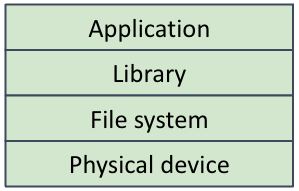
\includegraphics[width=0.95\textwidth]{chapters/L6/images/layers.png}
\end{center}
\end{minipage}

\newpage
\subsubsection{Man Pages}
\textit{We'll take a further look at this during the project's warmup}\\
\textit{Man pages}, short for manual pages, are built-in documentation for Unix-like operating systems, providing detailed information about commands, system calls, functions, and files. Each man page typically includes a synopsis, description, options, usage examples, and related commands.

To access a man page, use the command:
\begin{center}
\begin{verbatim}
man [section] command
\end{verbatim}
\end{center}

For instance, the command:
\begin{center}
\begin{verbatim}
man fread
\end{verbatim}
\end{center}

shows documentation for the \texttt{fread} function, typically in the default section. However, since the same name may exist in multiple sections, specifying a section number can be necessary:

\begin{center}
\begin{verbatim}
man 3 fread
\end{verbatim}
\end{center}

explicitly requests documentation from section 3, which covers library functions (part of \texttt{libc}). \texttt{fread} and other \texttt{FILE*} calls offer benefits such as portability across operating systems and higher-level abstractions like buffering.

On the other hand, system calls, such as:
\begin{center}
\begin{verbatim}
man 2 read
\end{verbatim}
\end{center}

provide lower-level interfaces. The \texttt{read} system call, documented in section 2, directly uses file descriptors, allowing the same code to interact uniformly with files, pipes, and sockets (covered further in networking lectures).\newpage
\begin{example}[Example: Reading file contents in C (simplified \texttt{cat})]
\leavevmode
\upshape
This example illustrates how to implement a simple version of the \texttt{cat} command in C. It includes argument handling (\texttt{argv}), file I/O operations, writing to standard output (\texttt{stdout}), and briefly mentions how the tool \texttt{strace} can be used to trace system calls.

\begin{cc}
/*cat -- simplified -- */
#include <stdio.h>
#include <stdlib.h>

#define BUFSIZE (32*1024) // 32 KB buffer

int main(int argc, char *argv[]) {
    FILE *finput;
    char buf[BUFSIZE];
    size_t bsize;

    if (argc > 1) {
        // Open file in read-only mode
        finput = fopen(argv[1], "r");
        if (!finput) {
            perror("fopen");
            return 1;
        }

        do {
            bsize = fread(buf, 1, BUFSIZE, finput);
            if (bsize > 0)
                fwrite(buf, 1, bsize, stdout);
        } while (bsize == BUFSIZE);

        fclose(finput);
    } else {
        fprintf(stderr, "Usage: %s <file>\n", argv[0]);
        return 1;
    }

    return 0;
}
\end{cc}
\textbf{Compilation and Redirection}\\
To compile and run the simplified \texttt{cat} program:

\begin{lstlisting}[language=bash]
cc cat.c -o cat
./cat myfile.txt > output.txt
\end{lstlisting}

This illustrates the use of the indirection operator (\texttt{>}), redirecting the program's standard output to the file \texttt{output.txt}.

\textbf{System Call Tracing (\texttt{strace})}\\
You can trace system calls using \texttt{strace}:
\begin{lstlisting}[language=bash]
strace ./cat myfile.txt > output.txt
\end{lstlisting}
This will display all the system calls (such as \texttt{open}, \texttt{read}, and \texttt{write}) that the simplified \texttt{cat} program makes.
\end{example}
\newpage
\section{File System Goals and Core Components}
A file system provides reliable, long-term storage of information and is responsible for managing how data is stored and retrieved on secondary storage devices. Its primary goals are:

\begin{itemize}
    \item[-] \textbf{Persistent Storage}: Data remains stored across reboots and system shutdowns.
    \item[-] \textbf{Concurrent Access}: Allows simultaneous reading and writing by multiple processes.
    \item[-] \textbf{Human-Readable Naming}: Facilitates logical naming and organization of data for ease of access.
\end{itemize}

The file system comprises two fundamental components:
\begin{enumerate}
    \item \textbf{Files}
    \item \textbf{Directories}
\end{enumerate}

\subsection{Defining a File}

\begin{definition}[File]
A file is a named, persistent collection of related information stored on secondary storage, represented as a linear array of bytes.
\end{definition}

A file consists of two distinct components:

\begin{itemize}
  \item[-] \textbf{Data}: The content provided by users or applications, structured as a linear array of bytes.
  \item[-] \textbf{Metadata}: Auxiliary information managed by the operating system, including attributes such as:
    \begin{itemize}
        \item Size
        \item Ownership and permissions
        \item Modification and access timestamps
    \end{itemize}
\end{itemize}

\subsection{Perspectives on Files}
Files can be understood from three perspectives:
\begin{enumerate}
    \item \textbf{User Perspective (Human-readable paths)}
    \item \textbf{Operating System Perspective (Inode identification)}
    \item \textbf{Process Perspective (File descriptors)}
\end{enumerate}
\newpage

\subsection{User View: File Names}
From a user's perspective, files are identified using meaningful, human-readable names. Files are organized hierarchically within directories, allowing intuitive and logical structuring.\\[5px]
\begin{definition}[File Path]
A file path describes the location of a file within the hierarchical directory structure, uniquely identifying it within the entire file system.
\begin{itemize}
    \item[-] Filenames are unique within their local directory.
    \item[-] Full paths, however, provide globally unique identification.
\end{itemize}
\end{definition}

\subsubsection{File Content and Types}
Modern file systems primarily handle files as \textbf{untyped sequences of bytes}. The content interpretation is left entirely to the user applications; the OS neither understands nor manages content semantics.

\subsection{Operating System View: Inodes}
\begin{definition}[Inode]
  An inode (Index Node) is a low-level persistent data structure maintained by the file system. It contains metadata about a file and pointers to the data blocks on disk. \\[5px]
\end{definition}
\noindent
\begin{minipage}[htp]{0.45\textwidth}
\textbf{Characteristics of inodes}
\begin{itemize}
    \item[-] Each file is associated with exactly one inode.
    \item[-] Inode IDs are unique within the file system but not globally.
    \item[-] After deletion, inode numbers can be recycled and reassigned.
\end{itemize}
\end{minipage}%
\hfill
\vline
\hfill
\begin{minipage}[htp]{0.45\textwidth}
\textbf{Metadata stored in an inode}
\begin{itemize}[itemsep=3pt, topsep=1pt]
  \item[-] File permissions and ownership
  \item[-] File size
  \item[-] Timestamps (creation, modification, and access times)
  \item[-] Pointers to the actual data blocks and indirect blocks on storage media
\end{itemize}
\end{minipage}

\subsubsection{Management of Inodes by File Systems}
The file system dedicates a specific area of the disk known as the \textbf{inode table}, analogous to a linear page table, to manage inodes:
\begin{itemize}[itemsep=3pt, topsep=1pt]
  \item[-] The disk is partitioned into two distinct regions: one for inode tables and another for data blocks.
  \item[-] Each inode has a fixed, unique location within this inode table.
  \item[-] The inode number directly identifies the location of an inode on disk.
\end{itemize}
Typically, inode tables reside in a reserved area at the beginning of the storage medium.
\newpage
\subsection{Mapping Paths to Inodes}
File systems store mappings from human-readable filenames to inodes within special files known as \textbf{directories}.\\[3px]

\begin{definition}[Directory]\leavevmode \\[5px]
A directory is a special type of file containing an array of mappings between filenames and inode numbers.
\end{definition}


\begin{example}[Resolving a path]
\leavevmode
\\[5px]
Resolving a path to its corresponding inode involves sequentially traversing directories:\\
\noindent
\begin{minipage}{0.45\textwidth}
Accessing the file \texttt{/tmp/test.txt} involves three steps
\begin{enumerate}
    \item Locate the inode of directory \texttt{tmp} in the root directory (\texttt{/}).
    \item Within \texttt{tmp}, find the inode associated with \texttt{test.txt}.
    \item Access the file content via the identified inode.
\end{enumerate}
\end{minipage}%
\hfill
\vline
\hfill
\begin{minipage}{0.45\textwidth}
\begin{center}
  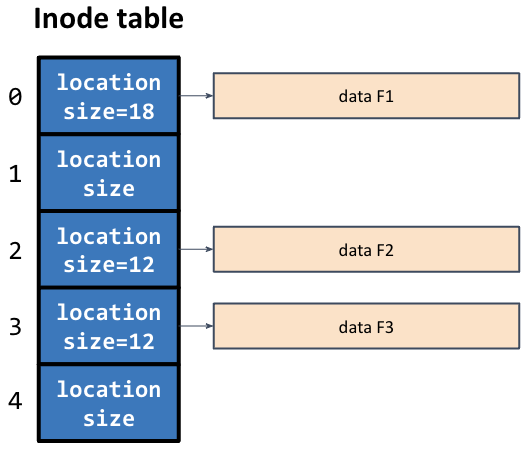
\includegraphics[width=0.95\textwidth]{chapters/L6/images/inode-table.png}
\end{center}
\end{minipage}
\end{example}

\subsubsection{Relationship Between Inodes and Directories}
Important distinctions regarding directories and inodes:
\begin{itemize}
  \item[-] Directories themselves are stored as regular files but with a special identifying flag.
  \item[-] This special flag restricts operations (e.g., writing directly to directory files is prohibited).
  \item[-] Directories contain arrays of pairs \texttt{\{filename, inode number\}}.
  \item[-] An inode does \textbf{not} store its filename; filenames are only stored in directory entries.
\end{itemize}

\newpage
\subsection{Directory Organization}
The file system organizes data into directories and files with a hierarchical structure. 
\begin{center}
  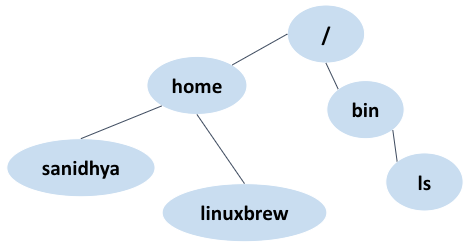
\includegraphics[width=0.45\textwidth]{chapters/L6/images/file-tree.png}
\end{center}
\begin{itemize}
  \item[-] \textbf{Root Directory:} Denoted by ``/'' (typically associated with inode 1).
  \item[-] \textbf{Navigation:}
    \begin{itemize}
      \item[-] ``.'' refers to the current directory.
      \item[-] ``..'' refers to the parent directory.
    \end{itemize}
\end{itemize}
\begin{center}
  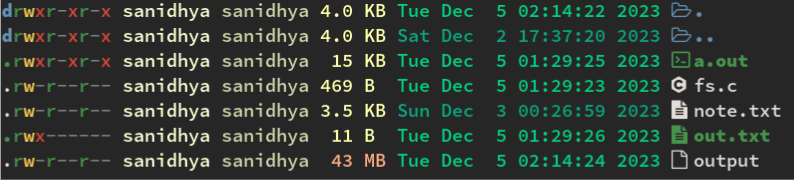
\includegraphics[width=0.45\textwidth]{chapters/L6/images/permissions.png}
\end{center}
\begin{itemize}
  \item[-] \textbf{Permission Bits:} Each file or directory has nine permission characters following a leading type indicator (e.g., ``d'' for directory or ``-'' for file):
    \begin{itemize}
      \item[-] \textbf{Owner:} Read, write, and execute (rwx).
      \item[-] \textbf{Group:} Typically read and execute (r-x).
      \item[-] \textbf{Others:} Typically read and execute (r-x).
    \end{itemize}
    \begin{itemize}
      \item[-] For files, the execute bit (``x'') indicates that the file is executable.
      \item[-] For directories, the execute bit allows users to change into the directory (i.e., using \texttt{cd}).
    \end{itemize}
\end{itemize}



\subsection{File Referencing via Links}
Links provide a means to reference a file by its location or name without duplicating its data. There are two primary types of links:

\begin{description}
  \item\textbf{Hard Links}
    \begin{itemize}
      \item[-] Associate an alternative file name directly with the same inode as the original file.
      \item[-] Serve as mirror copies; both names refer to the same underlying data.
      \item[-] Deleting one hard link does not remove the actual data as long as another hard link exists.
    \end{itemize}
    
  \item\textbf{Symbolic (Soft) Links}
    \begin{itemize}
      \item[-] Create a reference by logically mapping a file path to a target file.
      \item[-] Allocate a new inode for the link.
      \item[-] If the target file is removed, the symbolic link becomes broken or invalid.
    \end{itemize}
\end{description}

\subsection{Process View: File Descriptors}
File system operations can be implemented using file names along with inode and device IDs.\\ However, performing a lookup from a file name to its corresponding inode/device ID for every operation can be inefficient.\\
To overcome this, most systems perform the expensive directory traversal once and then store the resulting inode/device number in a per-process table known as the file descriptor (fd) table. \\

This table not only holds the inode/device number but also maintains additional information such as the current file offset. File descriptors are represented by small non-negative integers (typically 0, 1, 2, etc.) and are reused when they are freed.

\begin{example}[Operations on a File]
\leavevmode
\\[5px]
\noindent
\begin{minipage}{0.45\textwidth}
Each process maintains its own file descriptor table. The first three descriptors are reserved:
\begin{itemize}
  \item[] \textbf{0:} Standard Input (STDIN)
  \item[] \textbf{1:} Standard Output (STDOUT)
  \item[] \textbf{2:} Standard Error (STDERR)
\end{itemize}
For example, a file opened by a process might receive file descriptor 3 (with an associated inode, say X). When a read operation is performed, the file offset is updated (e.g., from 0 to 23). If another descriptor (say, file descriptor 4) is assigned to the same file, it starts with its own independent offset (e.g., initialized to 0).
\end{minipage}%
\hfill
\vline
\hfill
\begin{minipage}{0.45\textwidth}
\begin{center}
  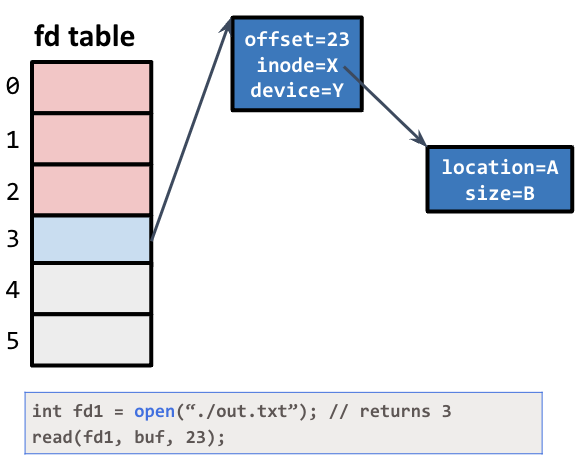
\includegraphics[width=1\textwidth]{chapters/l6/images/ops.png}
\end{center}
\end{minipage}
\end{example}

\newpage

\section{File System API}
The File System API in UNIX-like operating systems provides a set of system calls to manage files programmatically. This section introduces essential operations such as creating, opening, closing, reading, writing, and manipulating file metadata.

\subsubsection{Creating and Opening Files}
To create or open a file, the \texttt{open()} system call is utilized:
\begin{cc}
int open(const char *pathname, int flags, mode_t mode);
\end{cc}
\begin{itemize}[itemsep=3pt, topsep=3pt]
  \item[-] \texttt{pathname}: Path to the file.
  \item[-] \texttt{flags}: Define the access mode and creation flags.
  \item[-] \texttt{mode}: Set permissions for the file, effective when \texttt{O\_CREAT} is specified.
  \item[-] Returns a file descriptor (fd), a non-negative integer used to perform subsequent operations.
\end{itemize}

\begin{example}[Creating and opening a file]
The following code snippet demonstrates creating a file named \texttt{"out.txt"} with read, write, and execution permissions for the owner:
\begin{cc}
int fd = open("./out.txt", O_CREAT | O_RDWR | O_TRUNC, S_IRWXU);
\end{cc}
\end{example}

\subsubsection{Closing Files}

Files should be explicitly closed using the \texttt{close()} system call to release resources:

\begin{cc}
int close(int fd);
\end{cc}
\begin{itemize}[itemsep=2pt, topsep=1pt]
  \item[-] \texttt{fd}: File descriptor.
  \item[-] Returns 0 on success, or -1 on failure.
\end{itemize}

\subsubsection{Reading and Writing Data}

The File System API provides two primary system calls to perform I/O operations:

\begin{cc}
ssize_t read(int fd, void *buffer, size_t count);
ssize_t write(int fd, const void *buffer, size_t count);
\end{cc}
\begin{itemize}[itemsep=2pt, topsep=1pt]
  \item[-] \texttt{fd}: File descriptor.
  \item[-] \texttt{buffer}: Memory area for input/output data.
  \item[-] \texttt{count}: Number of bytes to read/write.
  \item[-] Both calls return the number of bytes successfully processed.
\end{itemize}
\newpage
\subsubsection{Managing File Offset}

To manipulate the file offset explicitly, use the \texttt{lseek()} system call:

\begin{cc}
off_t lseek(int fd, off_t offset, int whence);
\end{cc}
\begin{itemize}[itemsep=2pt, topsep=1pt]
  \item[-] \texttt{fd}: File descriptor.
  \item[-] \texttt{offset}: Number of bytes to move.
  \item[-] \texttt{whence}: Position from which offset is applied:
    \begin{itemize}[itemsep=2pt, topsep=1pt]
      \item[-]\texttt{SEEK\_SET}: Beginning of file.
      \item[-] \texttt{SEEK\_CUR}: Current offset.
      \item[-] \texttt{SEEK\_END}: End of file.
    \end{itemize}
  \item[-] Returns the resulting offset location, or -1 on error.
\end{itemize}

\subsubsection{Deleting Files}

To remove a file, the \texttt{unlink()} system call is used:

\begin{cc}
int unlink(const char *pathname);
\end{cc}
\begin{itemize}[itemsep=2pt, topsep=1pt]
  \item[-] Removes file entry from the filesystem, reducing its reference count.
  \item[-] File is physically deleted when its reference count reaches zero.
\end{itemize}

\subsubsection{Synchronizing Data}

To ensure that all buffered data is written to disk, the \texttt{fsync()} system call is essential:

\begin{cc}
int fsync(int fd);
\end{cc}
\begin{itemize}[itemsep=2pt, topsep=1pt]
  \item[-] Flushes file data and metadata from memory to disk.
\end{itemize}

\subsubsection{Accessing File Metadata}
File metadata such as permissions, inode number, and timestamps can be retrieved using the \texttt{fstat()} system call:

\begin{cc}
int fstat(int fd, struct stat *statbuf);
\end{cc}
\begin{itemize}[itemsep=2pt, topsep=1pt]
  \item[-] Populates the provided \texttt{statbuf} structure with metadata.
  \item[-] Information retrieved includes device ID, inode number, permission bits, user ID, etc.
  \item[-] Returns 0 on success or -1 on failure.
\end{itemize}

\newpage
\begin{example}[Basic File Operations]
  \leavevmode \\[5px]
\upshape
The following program demonstrates a sequence of file operations:
\begin{cc}
#include <stdio.h>
#include <stdlib.h>
#include <string.h>
#include <unistd.h>
#include <fcntl.h>

int main() {
    int fd = open("./out.txt", O_CREAT | O_RDWR | O_TRUNC, S_IRWXU);

    char buffer[20] = {0};

    write(fd, "hello world", 11);      // Writes 11 bytes, offset at 11
    lseek(fd, 0, SEEK_SET);            // Resets offset to beginning

    read(fd, buffer, 5);               // Reads 5 bytes into buffer
    printf("Read data: %s\n", buffer); // Prints "hello"

    close(fd);                         // Closes the file descriptor
    return 0;
}
\end{cc}
\end{example}

\section{Mount Points}
Mountpoints are directory locations in a filesystem where storage devices or partitions are attached, allowing access to their contents.
\subsection{Multiple File Systems}
A single operating system may contain multiple file systems coming from different sources.\\
\begin{itemize}[itemsep=2pt, topsep=1pt]
    \item[-]Different partitions on the same physical disk
    \item[-]Multiple physical disks
    \item[-]Removable media such as DVD or Blu-ray drives
    \item[-]USB flash drives
    \item[-]Network Attached Storage (NAS)
    \item[-]Legacy devices such as floppy drives
\end{itemize}

This raises an important question: how do we organize, manage, and present these diverse file systems to users in a coherent manner?

The solution adopted by modern operating systems is to map all file systems into a single, unified hierarchy rooted at a common point:
\begin{description}
    \item[-][Windows:] File systems are mapped using drive letters (e.g., \texttt{C:\textbackslash}, \texttt{D:\textbackslash}).
    \item[-][Unix/Linux:] File systems can be mounted into any directory, integrating seamlessly into a single hierarchical tree. For instance, the directory \texttt{/home} can itself represent a separate file system.
\end{description}

The act of \textbf{mounting} integrates multiple distinct file systems across different storage devices into one logical structure accessible via the standard directory tree.
\newpage
\subsection{Benefits of Using Mount Points}
Using mount points provides several key advantages:
\begin{itemize}[itemsep=2pt, topsep=1pt]
    \item[-] A unified namespace offering a consistent view of all storage resources.
    \item[-] Uniform access through the same file system interface and API.
\end{itemize}

Common commands related to mounting in Unix/Linux environments include:
\begin{itemize}
    \item[-] \texttt{mount <device> <directory>}\quad (general syntax)
    \item[-] \texttt{mount /dev/cdrom /media/cdrom}\quad (example for mounting optical media)
    \item[-] \texttt{mount -t ext4 /dev/sda5 /home}\quad (mounting a specific file system type)
    \item[-] \texttt{df}\quad (reports disk space usage for all mounted file systems)
    \item[-] \texttt{df .}\quad (reports disk space usage for the current file system)
\end{itemize}

\section{From File System Abstraction to Implementation}
\subsection{File System Implementation}
A file system manages and organizes user data efficiently on storage media. To achieve this, the following elements must be considered:

\begin{itemize}[itemsep=2pt, topsep=1pt]
    \item[-] \textbf{Storage Structure:} Typically represented as a large sequence of $N$ storage blocks.
    \item[-] \textbf{Metadata Organization:} Data structures that clearly encode file hierarchies and individual file metadata.
    \item[-] \textbf{Efficiency Criteria:}
    \begin{itemize}
        \item[-] Minimize metadata overhead compared to actual file data.
        \item[-] Minimize internal fragmentation (unused space within allocated blocks).
        \item[-] Provide efficient access to file contents, reducing external fragmentation and metadata access overhead.
    \end{itemize}
    \item[-] \textbf{Implementation of File System APIs:} Offers multiple design choices analogous to virtual memory implementations.
\end{itemize}

\subsection{File System Layout on Disk}

The file system is physically stored on disk drives, which are typically structured into partitions. The primary layout includes:
\begin{center}
  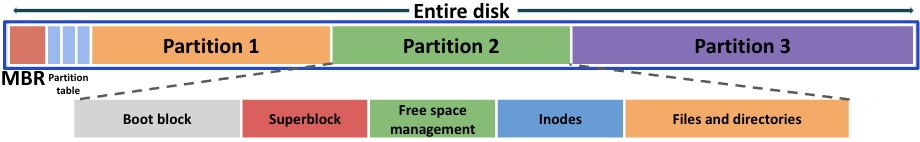
\includegraphics[width=0.8\textwidth]{chapters/L6/images/fs-layout-ondisk.png}
\end{center}


\textbf{Disk Structure}\\
\begin{itemize}[itemsep=2pt, topsep=1pt]
    \item[-] \textbf{Sector 0 (Master Boot Record - MBR):}
\begin{itemize}[itemsep=2pt, topsep=1pt]
        \item[-] Contains bootstrap code executed by firmware during startup.
        \item[-] Stores a partition table indicating partition boundaries.
    \end{itemize}
    \item[-] \textbf{Boot Block:} Located at the start of each partition, it contains executable boot code loaded by the MBR.
\end{itemize}

\subsection{Detailed View: Inside a Partition}
Each partition is structured into a sequential collection of blocks:
\begin{center}
     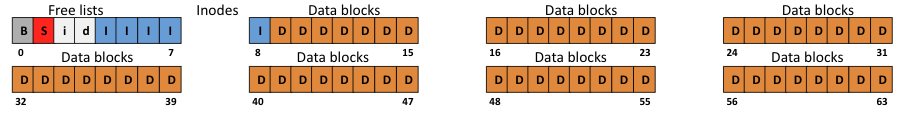
\includegraphics[width=1\textwidth]{chapters/L6/images/storage-block.png}
\end{center}

\textbf{Partition Structure}\\
\begin{itemize}[itemsep=2pt, topsep=1pt]
      \item[-] \textbf{Block Organization:} Blocks numbered from $0$ to $N-1$ (e.g., 64 blocks, each of 4KB).
      \item[-] \textbf{Block Types:}
      \begin{itemize}
          \item[-] \textit{Data Blocks}: Contain actual file content.
          \item[-] \textit{Metadata Blocks}: Manage file system structure, including:
          \begin{itemize}
              \item[-] An array of \textit{inodes} (file descriptors).
              \begin{itemize}
                  \item[-] Example: If an inode size is 256 bytes, each 4KB block can store 16 inodes. Thus, 5 blocks provide space for up to 80 files.
              \end{itemize}
              \item[-] Bitmap structures or free lists that track available inodes and data blocks.
          \end{itemize}
      \end{itemize}
      \item[-] \textbf{Boot and Superblock:} Typically placed at the beginning of each partition for initialization and file system configuration.
  \end{itemize}


This layout ensures systematic management of storage, facilitating efficient data retrieval and minimizing fragmentation.

\subsection{File System Superblock}
The file system superblock stores critical metadata describing the structure and organization of the file system. Key characteristics include:
\begin{itemize}[itemsep=2pt, topsep=1pt]
    \item[-] Exists as one logical superblock per file system.
    \item[-] Contains essential metadata, such as:
    \begin{itemize}
        \item[-] Number of inodes
        \item[-] Number of data blocks
        \item[-] Location of the inode table
        \item[-] Information to track free inodes and data blocks
    \end{itemize}
    \item[-] The first structure read when mounting the file system.
\end{itemize}
\newpage
\subsection{File Inode}
An inode is a data structure used to store metadata about an individual file or directory. Typical inode attributes include:
\begin{itemize}[itemsep=2pt, topsep=1pt]
    \item[-] File type (regular file, directory, symbolic link)
    \item[-] User ID of the owner
    \item[-] Permissions (Read/Write/Execute)
    \item[-] File size in bytes
    \item[-] Block addresses containing the file's data
    \item[-] Creation timestamp
    \item[-] Number of linked paths (hard links)
    \item[-] Counts of direct and indirect data blocks
\end{itemize}

\subsection{File Allocation Methods}
File allocation methods determine how files are stored on disk blocks. The following approaches are commonly used:

\begin{itemize}[itemsep=2pt, topsep=1pt]
    \item[-] \textbf{Contiguous Allocation}: Files stored in sequential blocks.
    \item[-] \textbf{Linked Allocation}: Files stored as linked lists of blocks.
    \item[-] \textbf{File Allocation Table (FAT)}: Uses a central table to manage file blocks.
    \item[-] \textbf{Multi-level Indexed Allocation}: Files managed through hierarchical index pointers.
\end{itemize}

The choice of allocation method depends on considerations such as fragmentation, access patterns, metadata overhead, and file growth or shrinkage requirements.

\begin{center}
    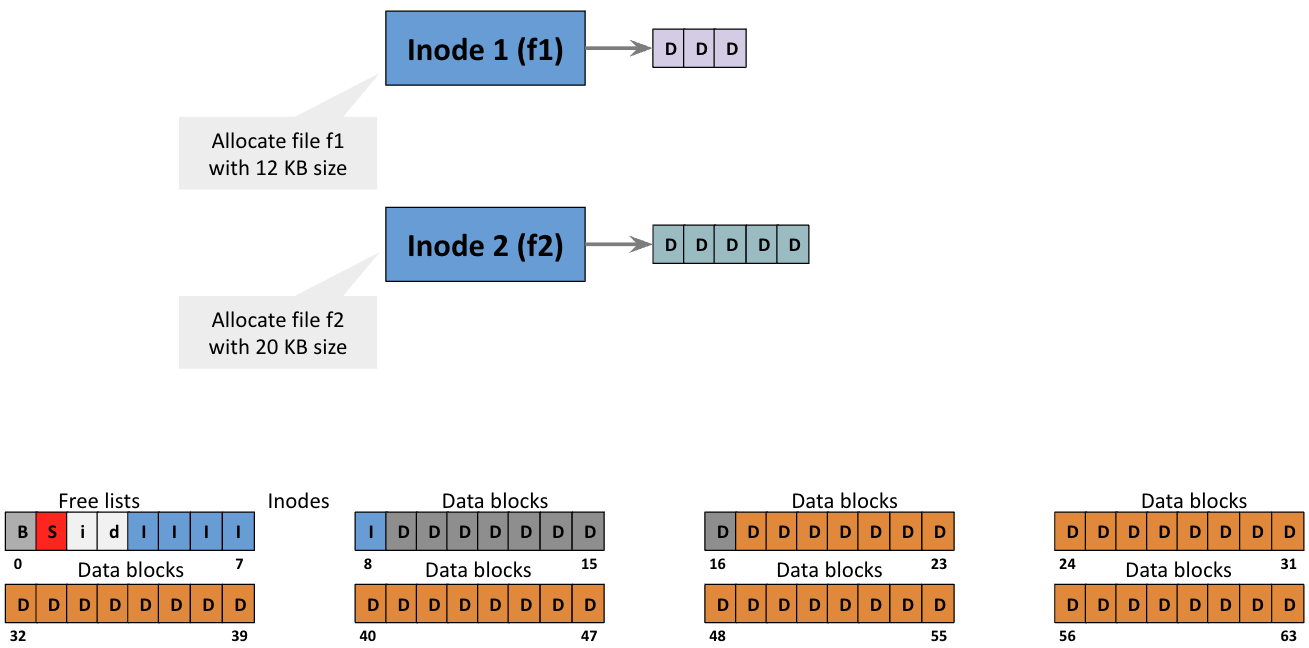
\includegraphics[width=0.95\textwidth]{chapters/L6/images/alloc.png}
\end{center}
\newpage
\subsection{Contiguous Allocation}
In contiguous allocation, all blocks of a file are stored consecutively on disk.
\begin{center}
  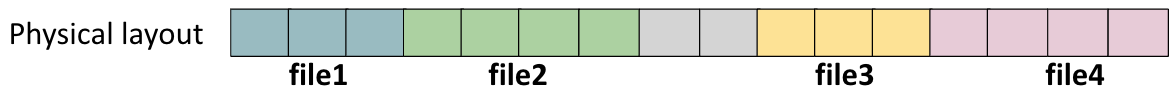
\includegraphics[width=0.95\textwidth]{chapters/L6/images/contiguous.png}
\end{center}


\begin{itemize}[itemsep=2pt, topsep=1pt]
    \item[-] \textbf{Simplicity}: Requires only the starting block and file length.
    \item[-] \textbf{Efficiency}: Fast sequential and random access (one seek operation for entire file).
    \item[-] \textbf{Fragmentation}: Susceptible to external fragmentation, especially when files are frequently created and deleted.
    \item[-] \textbf{Limitations}: Difficult to resize files; file size must be known at creation.
    \item[-] \textbf{Typical Use}: Ideal for read-only media (e.g., CD/DVD/Blu-ray).
\end{itemize}

\subsection{Linked Allocation}
In linked allocation, each file is stored as a linked list of disk blocks. Each block contains data and a pointer to the next block.
\begin{center}
  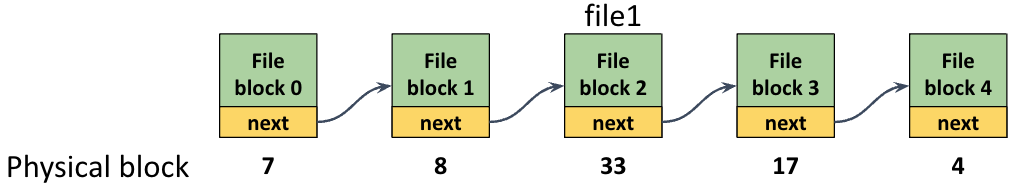
\includegraphics[width=0.85\textwidth]{chapters/L6/images/linked.png}
\end{center}
\begin{itemize}[itemsep=2pt, topsep=1pt]
    \item[-] \textbf{Space Utilization}: Eliminates external fragmentation.
    \item[-] \textbf{Simplicity}: Only starting block needed to access the file.
    \item[-] \textbf{Performance}: Efficient sequential access, but poor random access.
    \item[-] \textbf{Overhead}: Metadata overhead due to pointers in each block.
    \item[-] \textbf{Implementation}: Data and metadata (pointers) are mixed in each block.
\end{itemize}

\newpage

\subsection{File Allocation Table (FAT)}
The FAT system decouples data from metadata by using a centralized table containing block references. Each table entry points to the next block of the file.
\begin{center}
  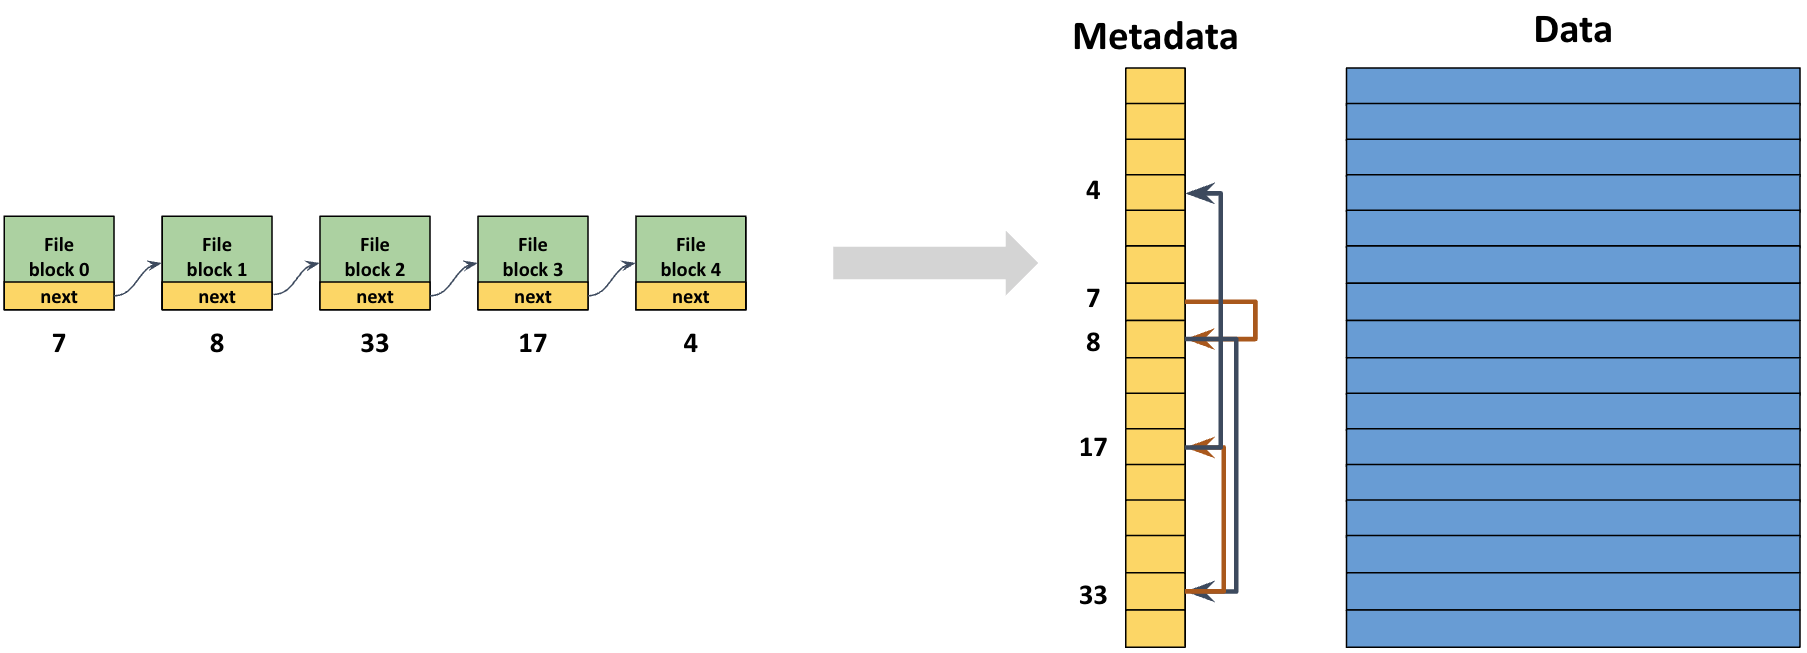
\includegraphics[width=1.05\textwidth]{chapters/L6/images/fat.png}
\end{center}
\begin{itemize}[itemsep=2pt, topsep=1pt]
    \item[-] \textbf{Structure}: Centralized table separates pointers (metadata) from data blocks.
    \item[-] \textbf{Fragmentation}: Avoids external fragmentation.
    \item[-] \textbf{Simplicity}: File access requires only the starting block index.
    \item[-] \textbf{Performance}: Good sequential access, but slower random access due to indirect lookups.
    \item[-] \textbf{Memory Overhead}: FAT can consume significant memory if not fully cached (e.g., 1GB for a 1TB disk with 4KB blocks).
\end{itemize}


\end{document}
